\documentclass[17pt,aspectratio=169]{beamer}

% packages
\usepackage{xcolor}
\usepackage{amsmath}
\usepackage{varwidth}
\usepackage{graphicx}
\usepackage{enumerate}
\usepackage{makecell}
\usepackage{tcolorbox}
\usepackage{xfrac}
\usepackage{fp}
\usepackage{xfp}
\newcommand{\modulo}[2]{%
  \FPeval{\result}{trunc(#1-(#2*trunc(#1/#2,0)),0)}\result%
}


% references
\renewcommand*{\thefootnote}{\fnsymbol{footnote}}

\usepackage[doi=false,isbn=false,url=false,eprint=false,date=year,
maxbibnames=1,maxnames=2,giveninits=true,
citestyle=alphabetic, bibstyle=alphabetic]{biblatex}
\addbibresource{references.bib}
\renewbibmacro{in:}{}

\AtBeginEnvironment{frame}{\setcounter{footnote}{0}}

\setbeamercolor{bibliography entry author}{fg=purple}
\setbeamercolor{bibliography entry note}{fg=black}
\AtEveryCitekey{\iffootnote{\scriptsize}{}}

\usepackage{tikz}
\usetikzlibrary{tikzmark}
\usetikzlibrary{shapes,snakes}
\usetikzlibrary{arrows.meta,arrows,bending}


\usepackage{shortcuts}

\definecolor{titlecolor}{rgb}{0.8, 0, 0.35}
\definecolor{emphcol}{rgb}{0.09, 0.45, 0.27}
% \definecolor{titlecolor}{rgb}{0.9, 0.28, 0.5}


% title page
\setbeamercolor{title}{fg=titlecolor}
\setbeamerfont{title}{size=\large}

% frametitle
\setbeamercolor{frametitle}{bg=white,fg=titlecolor}
\setbeamerfont{frametitle}{size=\LARGE}

% font
% \usefonttheme{serif} % default family is serif

% section slides
% \AtBeginSection[]{
%   \begin{frame}
%   \vfill
%   \centering
%   \begin{beamercolorbox}[sep=8pt,center,shadow=true,rounded=true]{title}
%     \usebeamerfont{title}Part \insertsectionnumber\\ -------------------------------------------- \\ \huge \insertsectionhead\par%
%   \end{beamercolorbox}
%   \vfill
% \end{frame}
% }

% remove navigation buttons
\beamertemplatenavigationsymbolsempty


% frame number
\setbeamerfont{footline}{size=\normalsize}
\setbeamertemplate{footline}{\hfill\Large\insertframenumber\hspace{0.3em}\vspace{0.5em}}%[frame number]

% itemize
\setbeamercolor{itemize item}{fg=titlecolor}
\setbeamercolor{itemize subitem}{fg=titlecolor}
\setbeamercolor{itemize subsubitem}{fg=titlecolor}
\setbeamertemplate{itemize items}{$\ast$}

\setbeamercolor{enumerate item}{fg=titlecolor}
\setbeamercolor{enumerate subitem}{fg=titlecolor}
\setbeamercolor{enumerate subsubitem}{fg=titlecolor}


\setbeamertemplate{frametitle}{
  \begin{center}
    \insertframetitle
  \end{center}
}


\title{\Large Exploiting Problem Structure in Privacy-Preserving
  Optimization and Machine Learning
}
\author{
  PhD Defense -- Paul Mangold\\[0.5em]
  \small Supervisors: Aurélien Bellet, Marc Tommasi
%  \small In collaboration with: Joseph Salmon, Michaël Perrot
  \vspace{-1em}
}

\date{October 11, 2023}

\begin{document}
{

\setbeamertemplate{footline}{}
\begin{frame}
  \titlepage
\end{frame}
}
\addtocounter{framenumber}{-1}

\begin{frame}{Let's Start with a Story}
  \pause
  \hspace{2em}%
  \begin{tikzpicture}
      \node[inner sep=0pt] (phone) at (0,0)
      {\includegraphics[width=.15\textwidth]{pics/malade.png}};
      \only<3>{
        \draw[->, line width=3mm] (1.5,0) -- (7,0);
        \node[inner sep=0pt] (phone) at (9,0)
        {
\includegraphics[width=.15\textwidth]{pics/hospital.pdf}};
      };
    \end{tikzpicture}
\end{frame}

% \begin{frame}
%   \begin{center}
%     \only<1>{\includegraphics[width=0.6\linewidth]{pics/sick.png}}
%     \only<2>{\includegraphics[width=0.6\linewidth]{temp_pics/fall.jpg}}
%     \only<3>{\includegraphics[width=0.6\linewidth]{temp_pics/goto_hospital.jpg}}
%   \end{center}
% \end{frame}

\begin{frame}{Let's Start with a Story}
  \begin{minipage}{0.3\linewidth}
    \begin{center}
      
\includegraphics[width=0.7\textwidth]{pics/hospital.pdf}
    \end{center}
  \end{minipage}%
  \begin{minipage}{0.7\linewidth}
    \begin{itemize}
      \pause
    \item Examination
      \pause
    \item Diagnosis
      \pause
    \item Cure
    \end{itemize}
  \end{minipage}
  \hspace{1em}

      \pause
      \vspace{0.5em}$\Rightarrow$ possible due to years of medical research

      \hspace{1em} (partly using statistical/machine learning)

\end{frame}

\begin{frame}
  \begin{minipage}{0.5\linewidth}

    \vspace{1em}

    \begin{table}
      \centering
      \scriptsize
      \begin{tabular}{c|ccccc}
       Record & \makecell{Age \\[-0.2em] $\color{black}x_1$} & \makecell{Pain \\[-0.2em] $\color{black}x_2$} & \makecell{$\dots$\\[-0.2em] \color{black} $\dots$} & \makecell{Drug \\[-0.2em] $\color{black}x_p$} & \makecell{Sick \\[-0.2em] $\color{black}y$} \\
        \hline
        \#1 & 27 & 1 & $\cdots$ & 1 & 1
        \\
        \#2 & 47 & 0 & $\cdots$ & 1 & 0
        \\
        \#3 & 52 & 0 & $\cdots$ & 0 & 0
        \\
        \#4 & 81 & 1 & $\cdots$ & 0 & 1
        \\
        $\cdots$ & $\cdots$ & $\cdots$ & $\cdots$ & $\cdots$ & $\cdots$
        \\
        \#n & 13 & 1 & $\cdots$ & 0 & 1
      \end{tabular}
    \end{table}
  \end{minipage}~~~~%
  \begin{minipage}{0.45\linewidth}
    How to study influence of

    possibly many features~$x_i$'s

    on an outcome~$y$?
  \end{minipage}

  \pause
  One way: model $\log (\tfrac{\prob(\text{sick})}{\prob(\text{not sick})})$ as
  \begin{align*}
    h_{w^*}(x) =  {\color{purple}w^*_0} + {\color{purple}w^*_1} \cdot x_1 + \cdots + {\color{purple}w^*_p} \cdot x_p
  \end{align*}

  \pause

  Core remark: $w^*$ is \bfseries{\color{purple} computed from the data}!

\end{frame}



\begin{frame}{$\boldsymbol{\Rightarrow}$ Trained Classification Model}
  \begin{minipage}{0.55\linewidth}
    \begin{center}
      \only<1>{\includegraphics[width=\linewidth]{img/logistic_reg_data.pdf}}
      \only<2,3>{\includegraphics[width=\linewidth]{img/logistic_reg_base.pdf}}
    \end{center}
  \end{minipage}~%
  \begin{minipage}{0.44\linewidth}
    \pause
    \pause

    \vspace{-1em}
    The resulting model:
    \begin{itemize}
    \item is (quite) accurate
    \item contains info on data
    \end{itemize}
  \end{minipage}

\end{frame}

\begin{frame}[t]{Two Societal Concerns}
  \setlength\leftmarginii{0em}
  \begin{enumerate}
  \item[\#1] Privacy of training data
    \begin{itemize}
      \addtolength{\leftmarginii}{15ex}
    \item guarantee that no confidential information is leaked
    \end{itemize}

    \vspace{1em}

  \item[\#2] Fairness of predictions
    \begin{itemize}
    \item guarantee similar predictions on all groups of population
    \end{itemize}
  \end{enumerate}
\end{frame}

\begin{frame}[t]{Privacy Issues}
  Membership inference \footfullcite{shokri2017Membership}:
  \begin{minipage}{0.5\linewidth}
    \vspace{1em}
    \begin{center}
      \addtolength{\leftmargini}{-1em}
      \begin{quote}
      `` \small determine whether a given record was part of a model’s
      training dataset \normalsize ``
      \end{quote}
    \end{center}
    \vspace{1.5em}
  \end{minipage}~~%
  \begin{minipage}{0.45\linewidth}
    \vspace{-2em}
    \begin{center}\pause
      \begin{overlayarea}{\textwidth}{5cm}
        \only<2>{
          \includegraphics[height=5cm]{img/logistic_reg_base.pdf}
        }
        \only<3>{
          \includegraphics[height=5cm]{img/logistic_reg_changed.pdf}
        }
      \end{overlayarea}
    \end{center}
  \end{minipage}

\end{frame}

\begin{frame}[t]{Guaranteeing Privacy}

  Perturb the linear predictor:
  {\small
  \only<1>{
    \begin{align*}
      h_{w^*}(x) = w_0^* + w^*_1 \cdot x_1 + \cdots + w^*_p \cdot x_p
    \end{align*}
  }
  \only<2,3,4>{
    \begin{align*}
      \!\!\!h_{w^*+{\color{purple}\eta}}(x) = (w_0^* + {\color{purple}\eta_0}) + (w^*_1 + {\color{purple}\eta_1}) \cdot x_1 + \cdots + (w^*_p + {\color{purple}\eta_p}) \cdot x_p
    \end{align*}
  }
}

\begin{overlayarea}{\textwidth}{3cm}
  \only<3,4>{
    \vcenteredinclude[width=.8cm]{pics/tick-mark-icon.pdf}
    noise gives \emph{plausible deniability} $\rightarrow$ better privacy

    \vspace{0.5em}

    \pause

    \vcenteredinclude[width=.8cm]{pics/incorrect-icon.pdf}
    noisy predictions $\rightarrow$ lower accuracy
    \vspace{0.5em}
  }
  \only<4>{
    \begin{center}
      \large
      $\boldsymbol{\Rightarrow}$ \bfseries\textcolor{purple}{tension between privacy and utility}
    \end{center}
  }
\end{overlayarea}

\end{frame}

\begin{frame}{How Strong is the Protection?}

  $\emphcolb{\cA} : D \mapsto w$ is
  $(\emphcol{\epsilon}, \emphcol{\delta})$-\emph{Differentially
    Private}\footfullcite{dwork2006Differential}
  \pause  \vspace{-1em}

  \begin{align*}
    \prob(\emphcolb{\cA}(D) \in \cS)
    \le
    \exp(\emphcol{\textcolor{purple}{\boldsymbol\epsilon}}) \cdot \prob(\emphcolb{\cA}(D') \in \cS) + \textcolor{purple}{\boldsymbol\delta}
  \end{align*}

  \vspace{1em}


  for \emph{all} $D, D'$ that differ on one element

  \vspace{1em}
  \pause

  Rule of thumb: $\textcolor{purple}{\boldsymbol\epsilon} \le 1$, $\textcolor{purple}{\boldsymbol\delta} = o(1/\abs{D})$

  \vspace{1em}


\end{frame}


\begin{frame}[t]{Two Societal Concerns}
  \setlength\leftmarginii{0em}
  \begin{enumerate}
  \item[\#1] Privacy of training data
    \begin{itemize}
      \addtolength{\leftmarginii}{15ex}
    \item guarantee that no confidential information is leaked
    \end{itemize}

    \vspace{1em}

  \item[\#2] Fairness of predictions
    \begin{itemize}
    \item guarantee similar predictions on all groups of population
    \end{itemize}
  \end{enumerate}
\end{frame}



\begin{frame}[t]{Fairness Issues}

  \vspace{-0.5em}

  \begin{minipage}{0.52\linewidth}
    \begin{center}
      \only<1>{\includegraphics[width=\linewidth]{img/logistic_reg_base.pdf}}%
      \only<2>{\includegraphics[width=\linewidth]{img/logistic_reg_base_fair.pdf}}%
      \only<3>{\includegraphics[width=\linewidth]{img/logistic_reg_base_shirt.pdf}}%
      \only<4>{\includegraphics[width=\linewidth]{img/logistic_reg_base_dress.pdf}}%
      \only<5>{\includegraphics[width=\linewidth]{img/logistic_reg_base_dress.pdf}}%
    \end{center}
  \end{minipage}~~%
  \begin{minipage}{0.4\linewidth}
    \textsc{Group Fairness}:
    \begin{center}
      \small
      Different groups can be treated differently
    \end{center}

    \pause%
    \pause%
    \pause%
    \pause%
    \vspace{0.5em}

  \end{minipage}

  \vspace{0.5em}
  \begin{overlayarea}{\textwidth}{3cm}
  \begin{center}
    Note: Perturbing the model can have a disparate impact\only<5>{\footfullcite{bagdasaryan2019Differential}}
  \end{center}
  \end{overlayarea}
\end{frame}

\begin{frame}
  \large

  \vspace{1em}

  How to exploit problem's structure to:

  \begin{center}
    \begin{itemize}
      \setlength{\itemsep}{0.5em}
    \item obtain better utility?
    \item study the impact of privacy on fairness?
    \end{itemize}

  \end{center}
\end{frame}

\begin{frame}{\textsc{Contributions}}
  \pause

  \settowidth{\leftmargini}{\usebeamertemplate{itemize item}}
  \begin{itemize}
    \large
  \item Private learning algorithms exploiting structure
    \begin{enumerate}
      \normalsize
    \item[1.] Imbalanced parameter scales and variations
    \item[2.] High-dimensional models with imbalanced solutions
    \end{enumerate}
    \vspace{1em}
    \pause
  \item Study interplay between privacy and fairness
    \large
    \begin{enumerate}
      \normalsize
    \item[3.] Bound on the impact of privacy on fairness
    \end{enumerate}
  \end{itemize}
\end{frame}

\begin{frame}{\textsc{Contributions}}

  \settowidth{\leftmargini}{\usebeamertemplate{itemize item}}
  \begin{itemize}
    \large
  \item Private learning algorithms exploiting structure
    \begin{enumerate}
      \normalsize
    \item[1.] Imbalanced parameter scales and variations
    \item[2.] High-dimensional models with imbalanced solutions
    \end{enumerate}
    \vspace{1em}
  \item[\textcolor{lightgray}{$\ast$}] \textcolor{lightgray}{Study interplay between privacy and fairness}
    \large
    \begin{enumerate}
      \normalsize
    \item[\textcolor{lightgray}{3.}] \textcolor{lightgray}{Bound on the impact of privacy on fairness}
    \end{enumerate}
  \end{itemize}
\end{frame}


\begin{frame}{Empirical Risk Minimization\\[-0.6em]\footnotesize \textcolor{gray}{Note: Most results also hold for composite ERM with Proximal algorithms}}
  \vspace{-1.5em}
  \begin{align*}
    w^* \in \argmin_{w \in \cW} \left\{ f(w) = \frac 1n \sum_{i=1}^n \ell(w; d_i) \right\}
  \end{align*}

  \pause

  \vspace{0.5em}

  \small
  Where $\cW \subseteq \RR^p$, has diameter $\norm{\cW}_2$, and $\ell$ is
  \begin{itemize}
    \setlength\itemsep{0.3em}
  \item \textcolor<2,4,5,6>{lightgray}{
      convex: $\ell(w;d) \ge \ell(w';d) + \langle \nabla \ell(w';d) , w - w' \rangle$
    }
  \item \textcolor<2,3,5,6>{lightgray}{
      smooth: $\norm{\nabla \ell(w; d) - \nabla \ell(w'; d)} \le M\norm{ w - w' }$
    }
    \item \textcolor<2,3,4>{lightgray}{
        Lipschitz:
        \only<2,3,4,5>{$\abs{\ell(w; d) - \ell(w'; d)} \le \Lambda \norm{w - w'}$}
        \only<6,7>{$\norm{\nabla \ell(w; d)} \le \Lambda$}
      }
  \end{itemize}

  \vspace{1em}

  \only<7>{
    \tikz[overlay,remember picture]
    \node[fill=white,text=black,draw=purple,fill=purple!5,inner sep=1.5cm, line width=1mm] at ([xshift=0cm,yshift=0cm]current page.center){
      {\LARGE \begin{varwidth}{\linewidth}How to solve ERM privately?\end{varwidth}}
    };
  }

\end{frame}

% \begin{frame}{SGD\\[-0.5em]\normalsize Stochastic Gradient Descent}
%   \begin{minipage}{0.6\linewidth}
%     \small
%    For $t = 0$ to $T-1$:
%     \begin{itemize}
%     \item Choose a data record $d_i$
%     \item Update
%       \begin{align*}
%         w^{t+1} = w^t -
%         \tikz[baseline,remember picture]{\node[fill=red!0,anchor=base] (step){$\gamma^t$};}
%         \!\!
%         \tikz[baseline,remember picture]{\node[fill=blue!0,anchor=base]
%         (grad){$\nabla\ell( w^t; d_i )$};}
%       \end{align*}
%     \end{itemize}
%     Return $w^T$

%   \end{minipage}~~~~%
%   \begin{minipage}{0.35\linewidth}
%     \vspace{1em}\only<2>{
%     \begin{center}
%       \tikz[remember picture,overlay]{\node[coordinate] (stepdef) {};}
%       \emph{uniform} step size $\gamma^t \propto 1/M$
%     \end{center}

%     \begin{center}

%       \tikz[remember picture,overlay]{\node[coordinate] (graddef) {};}
%       stochastic gradient

%       \vspace{-0.5em}
%       % \includegraphics[width=\linewidth]{temp_pics/gradient_imbalanced.jpg}
%       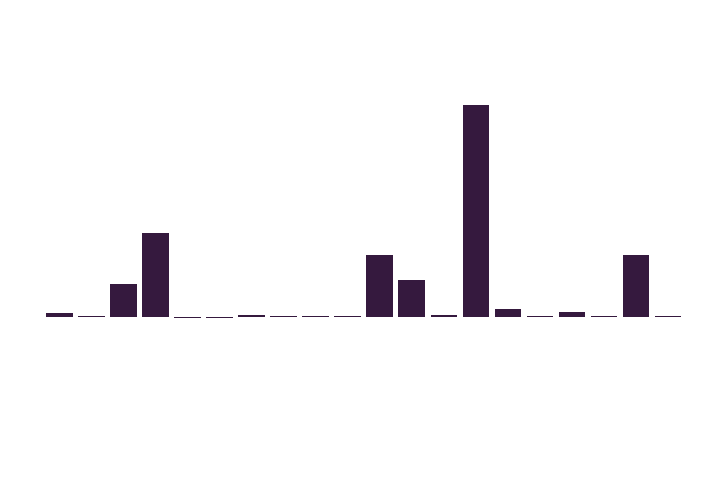
\includegraphics[width=\linewidth]{plots/grad_example_1.pdf}
%     \end{center}}
% \end{minipage}
% \only<2>{
%   \begin{tikzpicture}[remember picture,overlay]   %% use here too
%     \path[draw=magenta,thick,->] ([yshift=0.1cm]graddef.north) to [out=180, in=90,distance=0.5in] (grad.north);
%     \path[draw=magenta,thick,->] ([yshift=0.1cm]stepdef.north) to [out=180, in=90,distance=0.5in] (step.north);
%   \end{tikzpicture}
%   }


% \end{frame}


\begin{frame}{DP-SGD\footfullcite{song2013Stochastic}$^{,\hspace{0.1em}}$\footfullcite{bassily2014Private}\\[-0.5em]\normalsize Differentially Private Stochastic Gradient Descent}

  % \vspace{-0.3em}

%  \begin{minipage}{0.6\linewidth}
    \small
    For $t = 0$ to $T-1$:
    % \vspace{-0.5em}
    \begin{itemize}
    \item Choose a data record $d_i$
    \item Draw noise \textcolor{purple}{$\boldsymbol{\eta^t \sim \cN(0; \sigma^2\bbI_p)}$}
    \item Update
      $\displaystyle w^{t+1}
      = w^t -
      \tikz[baseline,remember picture]{\node[fill=red!0,anchor=base] (step){$\gamma^t$};}
      \!\!
      \tikz[baseline,remember picture]{\node[fill=blue!0,anchor=base]
        (grad){$(\nabla\ell( w^t; d_i ) + \textcolor{purple}{\eta^t})$};}
      $
    \end{itemize}
    % \vspace{-0.5em}
    Return $w^T$

%  \end{minipage}~~~~%
  % \begin{minipage}{0.35\linewidth}
  %   \vspace{1em}
  %   \begin{center}

  %   %   \tikz[remember picture,overlay]{\node[coordinate] (graddef) {};}
  %   %   \emph{noisy} stochastic gradient

  %   %   \vspace{-0.5em}
  %   %   % \includegraphics[width=\linewidth]{temp_pics/gradient_imbalanced.jpg}
  %   % \includegraphics[width=\linewidth]{plots/grad_example_noisy_1.pdf}
  %   \end{center}
  % \end{minipage}

%   \begin{tikzpicture}[remember picture,overlay]   %% use here too
%     \path[draw=magenta,thick,->] ([yshift=0.1cm]graddef.north) to [out=180, in=90,distance=0.5in] (grad.north);
% %    \path[draw=magenta,thick,->] ([yshift=0.1cm]stepdef.north) to [out=180, in=90,distance=0.5in] (step.north);
%   \end{tikzpicture}

  \vspace{1em}
\end{frame}

\begin{frame}{Privacy of DP-SGD\footfullcite{song2013Stochastic}$^{,\hspace{0.1em}}$\footfullcite{bassily2014Private}}

  % \vspace{-0.5em}

  % \begin{minipage}{0.6\linewidth}
  %   \small
  %   For $t = 0$ to $T-1$:
  %   \begin{itemize}
  %   \item Choose a data record $d_i$
  %   \item Draw noise \textcolor{purple}{$\eta^t \sim \cN(0; \sigma^2\bbI_p)$}
  %   \item Update

  %     $\displaystyle w^{t+1}
  %     = w^t -
  %     \tikz[baseline,remember picture]{\node[fill=red!20,anchor=base] (step){$\gamma^t$};}
  %     \tikz[baseline,remember picture]{\node[fill=blue!20,anchor=base]
  %       (grad){$(\nabla\ell( w^t; d_i ) + \textcolor{purple}{\eta^t})$};}
  %     $
  %   \end{itemize}
  %   \vspace{-0.5em}
  %   Return $w^T$

  % \end{minipage}~~~~%
  % \begin{minipage}{0.35\linewidth}
  For $(\epsilon,\delta)$-differential privacy we need

  \begin{align*}
    \sigma^2 = O\left(\frac{\Lambda T}{n^2 \epsilon^2}\right)
    \enspace,
    \enspace \enspace
    \text{where } \norm{\nabla \ell} \le \Lambda
  \end{align*}

  \vspace{0.5em}

  \begin{itemize}
  \item Noise increases with number of iterations
  \item Sampling amplifies privacy
  \end{itemize}

  \vspace{1em}
  % where $\norm{ \nabla \ell } \le \Lambda$
  % \end{minipage}
  % \vspace{1em}

\end{frame}

\begin{frame}{Utility of DP-SGD\footfullcite{bassily2014Private}}
  \begin{flalign*}
    \expec ( f(w^{SGD}) - f(w^*) )
    & =
      \only<1,2>{O}\only<3>{\boldsymbol{\color{purple}\Theta}}\Bigg(
      \only<1>{
      \tikz[baseline,remember picture]{\node[fill=red!20,anchor=base]
      (opt){$\displaystyle\tfrac{\Lambda \norm{\cW}_2}{\epsilon \sqrt{T}}$};}
      +
      \tikz[baseline,remember picture]{\node[fill=red!20,anchor=base]
      (priv){$\displaystyle\tfrac{\sqrt{T} p \Lambda \norm{\cW}_2 \log(1/\delta)}{n^2 \epsilon}$};}
      }
      \only<2,3>{
      \tikz[baseline,remember picture]{\node[fill=red!20,anchor=base]
      (balanced){$\displaystyle\tfrac{\Lambda \norm{\cW}_2 \sqrt{p\log(1/\delta)}}{n \epsilon}$};}
      }
      \Bigg)
    &&
  \end{flalign*}

  \vspace{1em}

  \only<1,2>{\vspace{0.2em}}%
  \only<1>{
    \qquad\qquad
    optimization error
    \tikz[remember picture,overlay]{\node[coordinate] (optdef) {};}
    \quad\quad
    privacy error
    \tikz[remember picture,overlay]{\node[coordinate] (privdef) {};}
  }
  \only<2>{
    ~~~~~~~~after balancing the two terms
    \tikz[remember picture,overlay]{\node[coordinate] (balanceddef) {};}
  }
  \only<3>{
    \begin{center}
      $\Rightarrow$ and the result is \emph{tight} (under these assumptions)
    \end{center}
  }

  \begin{tikzpicture}[remember picture,overlay]   %% use here too
    \only<1>{
      \path[draw=magenta,thick,->] ([yshift=0.1cm]optdef.east) to [out=0, in=-90,distance=0.5in] (opt.south);
      \path[draw=magenta,thick,->] ([yshift=0.1cm]privdef.east) to [out=0, in=-90,distance=0.5in] (priv.south);
    }
    \only<2>{
      \path[draw=magenta,thick,->] ([yshift=0.1cm]balanceddef.east) to [out=0, in=-90,distance=0.5in] (balanced.south);
    }
  \end{tikzpicture}

  \vspace{0.5em}  \only<1,2>{\vspace{0.6em}}%

\end{frame}

\begin{frame}{The Problem of DP-SGD\\[-0.5em]
  \normalsize \textcolor{gray}{It fails on imbalanced problems...}}
  \includegraphics[width=\linewidth]{img/1.pdf}
\end{frame}

\begin{frame}[t]
  \vspace{1em}

  We need to refine measure of regularity of $f$:
  \begin{itemize}
  \item \only<2,3>{\textcolor{purple}{coordinate-wise}} smoothness:
    \begin{align*}
      \only<1>{
      \norm{ \nabla f(w + t ) - \nabla f(w) }
      & \le M \norm{t}
      }
      \only<2,3>{
      \abs{ \nabla_{\boldsymbol{\textcolor{purple}{j}}} f(w + t e_{\boldsymbol{\textcolor{purple}{j}}}) - \nabla_{\boldsymbol{\textcolor{purple}{j}}} f(w) }
      & \le M_{\boldsymbol{\textcolor{purple}{j}}} \abs{t}
        }
    \end{align*}
  \item \only<2,3>{\textcolor{purple}{coordinate-wise}} Lipschitzness:
    \begin{align*}
      \only<1>{
      \norm{ \nabla f(w) }
      & \le \Lambda
      }
      \only<2,3>{
      \abs{ \nabla_{\boldsymbol{\textcolor{purple}{j}}} f(w) }
      & \le L_{\boldsymbol{\textcolor{purple}{j}}}
        }
    \end{align*}
  \end{itemize}

  \begin{overlayarea}{\textwidth}{5cm}
  \vspace{-1em}


    \only<3>{
      \vspace{0.5em}
      \begin{center}
        \tikz[baseline,remember picture]{\node[fill=red!20,anchor=base,inner sep=0.5cm]
          (important){
            Important: $M_{\boldsymbol{\textcolor{purple}{j}}} \le M$, and $L_{\boldsymbol{\textcolor{purple}{j}}} \le \Lambda$
          };}
      \end{center}
    }
  \end{overlayarea}

\end{frame}

\begin{frame}[t]
  We can now use a more appropriate measure of our space!

  \begin{center}
    \only<1>{\includegraphics[width=\linewidth]{img/1.pdf}}%
    \only<2,3>{\includegraphics[width=0.6\linewidth]{img/1_scaled.pdf}}
  \end{center}

  \begin{overlayarea}{\textwidth}{5cm}
  \only<3>{
    \begin{center}
      \small Scaled norm: $\displaystyle\norm{ w }_{M,q} = \Big( \sum_{{\boldsymbol{\textcolor{purple}{j}}}=1}^p M_{\boldsymbol{\textcolor{purple}{j}}}^{\tfrac{q}{2}}\abs{w_{\boldsymbol{\textcolor{purple}{j}}}}^q \Big)^{\tfrac{1}{q}}$ for $q \in \{1, 2\}$
    \end{center}
  }
  \end{overlayarea}
\end{frame}

\begin{frame}{Contribution 1: DP-CD\footfullcite{mangold2022Differentially} \\[-0.5em]
    \normalsize Differentially Private Coordinate Descent}
%  \vspace{1.5em}

  % \begin{minipage}{0.6\linewidth}
  % \vspace{-1em}
  \small
  For $t = 0$ to $T-1$:
%  \vspace{-0.5em}
  \begin{itemize}
    \setlength\itemsep{0.5em}
  \item Choose a \emph{coordinate ${\boldsymbol{\textcolor{purple}{j}}} \in [p]$}
  \item Draw noise
    \only<1>{$\eta_{\boldsymbol{\textcolor{purple}{j}}}^t \sim \cN\Big(0; \sigma_{\boldsymbol{\textcolor{purple}{j}}}^2\Big)$}%
    \only<2>{$\eta_{\boldsymbol{\textcolor{purple}{j}}}^t \sim \cN\Big(0; \boldsymbol{\textcolor{purple}{O\left(\frac{L_{\boldsymbol{\textcolor{purple}{j}}} T}{n^2 \epsilon^2}\right)}}\Big)$}%
  \item Update $w_{\boldsymbol{\textcolor{purple}{j}}}^{t+1} = w_{\boldsymbol{\textcolor{purple}{j}}}^t - \gamma_{\boldsymbol{\textcolor{purple}{j}}} ( \nabla_{\boldsymbol{\textcolor{purple}{j}}} f( w^t ) + \eta_{\boldsymbol{\textcolor{purple}{j}}}^t )$
  \end{itemize}
  \vspace{0.5em}

  Return $w^{CD} = \frac{1}{T} \sum_{t=1}^T w^t$
% \end{minipage}~~\pause%
% \begin{minipage}{0.35\linewidth}
%     For $(\epsilon,\delta)$-DP:
%     \begin{align*}
%       \sigma_{\boldsymbol{\textcolor{purple}{j}}}^2 = O\left(\frac{L_{\boldsymbol{\textcolor{purple}{j}}} T}{n^2 \epsilon^2}\right)
%     \end{align*}

%     where $\abs{ \nabla_{\boldsymbol{\textcolor{purple}{j}}}\ell } \le L_{\boldsymbol{\textcolor{purple}{j}}}$
% \end{minipage}

\vspace{0.9em}

\end{frame}

\begin{frame}
  \begin{minipage}{0.5\linewidth}
    % \only<1>{
    %   Non-private gradient:
    %   \begin{center}
    %     \includegraphics[width=0.9\linewidth]{img/normal_grad_nonoise.pdf}%
    %   \end{center}
    % }%
    % \only<2,3,4,5>{
    DP-SGD noise:
    \vspace{.2em}
    \begin{center}
      \includegraphics[width=0.9\linewidth]{img/normal_grad.pdf}%
    \end{center}
    % }
  \end{minipage}%
  \begin{minipage}{0.5\linewidth}
    DP-CD noise:
    \begin{center}
      % \only<3>{
      %   \includegraphics[width=0.9\linewidth]{img/normal_grad_gray.pdf}
      % }%
        \includegraphics[width=0.9\linewidth]{img/normal_grad_0.pdf}
    %   \only<2>{
    %     \includegraphics[width=0.9\linewidth]{img/normal_grad_10.pdf}
    %   }%
      \end{center}
  \end{minipage}
\end{frame}


\begin{frame}{Utility of DP-CD}
  \vspace{-1em}
  \begin{align*}
    \expec ( f(w^{CD}) - f(w^*) )
    & \le
      O \Bigg(
      \frac{ \sqrt{p \log(1/\delta) }  }{ n \epsilon } \norm{L}_{\boldsymbol{\textcolor{purple}{M^{-1}}}} \norm{ \cW }_{\boldsymbol{\textcolor{purple}{M}}}
      \Bigg)
  \end{align*}

  \vspace{1em}

  Recall that for DP-SGD:
  \begin{align*}
    \expec ( f(w^{SGD}) - f(w^*) )
    & \le
      O\Bigg(
      \frac{\sqrt{p\log(1/\delta)}}{n \epsilon} \Lambda \norm{\cW}_2
      \Bigg)
    &&
  \end{align*}
\end{frame}


\begin{frame}{Numerical Illustration\\[-0.5em]
  \only<1>{\normalsize \textcolor{gray}{DP-CD uses more appropriate step sizes}}
  \only<2>{\normalsize \textcolor{gray}{DP-CD does not require amplification by sampling}}
}
  \begin{minipage}{0.5\linewidth}
    \includegraphics[width=0.12\linewidth]{plots/xlegend.pdf}%
    \only<1>{\includegraphics[width=0.88\linewidth]{plots/optimization_electricity_simpler_raw.pdf}}%
    \only<2>{\includegraphics[width=0.88\linewidth]{plots/optimization_electricity_simpler_norm.pdf}}%
  \end{minipage}%
  \begin{minipage}{0.5\linewidth}
    \small
    \begin{itemize}
    \item Regularized logistic regression
    \item \only<1>{Raw (imbalanced) data}\only<2>{Standardized data}
    \item $n=45,312$ records
    \item $p=8$ features
    \item $\epsilon=1$, $\delta=1/n^2$
    \end{itemize}
  \end{minipage}

\end{frame}

\begin{frame}{Contribution 2: DP-GCD\footfullcite{mangold2023HighDimensional} \\[-0.5em]
    \normalsize Differentially Private {\bfseries{Greedy}} Coordinate Descent}

  \small

%  \begin{minipage}{0.65\linewidth}
  For $t = 0$ to $T-1$:
  \vspace{0.5em}
  \begin{itemize}
    \setlength\itemsep{0.5em}
  \item Draw noise $\eta_{\boldsymbol{\textcolor{purple}{j}}}^t, \zeta_{\boldsymbol{\textcolor{purple}{j}}}^t \sim \Lap\left(0; \boldsymbol{\textcolor{purple}{O\left(\frac{L_{\boldsymbol{\textcolor{purple}{j}}} T}{n^2 \epsilon^2}\right)}}\right)$
  \item Choose $\displaystyle {\boldsymbol{\textcolor{purple}{j}}} = \argmax_{{\boldsymbol{\textcolor{purple}{j}}}' \in [p]} \abs{ \nabla_{{\boldsymbol{\textcolor{purple}{j}}}'} f(w^t) + \zeta_{{\boldsymbol{\textcolor{purple}{j}}}'}}$

    \vspace{-0.5em}

  \item Update $w^{t+1} = w^t - \gamma_{\boldsymbol{\textcolor{purple}{j}}} ( \nabla_{\boldsymbol{\textcolor{purple}{j}}} f( w^t ) + \eta_{\boldsymbol{\textcolor{purple}{j}}}^t )$
  \end{itemize}

  \vspace{0.5em}

  Return $w^{GCD} = w^T$

%  \end{minipage}~~\pause%
  % \begin{minipage}{0.25\linewidth}
  %   For $(\epsilon,\delta)$-DP:
  %   \begin{align*}
  %     \lambda_{\boldsymbol{\textcolor{purple}{j}}}^2 = O\left(\frac{L_{\boldsymbol{\textcolor{purple}{j}}} T}{n^2 \epsilon^2}\right)
  %   \end{align*}

  %   where $\abs{ \nabla_{\boldsymbol{\textcolor{purple}{j}}}\ell } \le L_{\boldsymbol{\textcolor{purple}{j}}}$
  % \end{minipage}

  \vspace{1.1em}

\end{frame}


\begin{frame}
  \begin{minipage}{0.5\linewidth}
    DP-SGD noise:
    \begin{center}
      \includegraphics[width=0.9\linewidth]{img/normal_grad.pdf}%
%      \includegraphics[width=0.9\linewidth]{img/normal_grad_nonoise.pdf}%
    \end{center}
  \end{minipage}%
  \begin{minipage}{0.5\linewidth}
      % \only<1>{
      %   DP-CD noise:
      %   \begin{center}
      %     \includegraphics[width=0.9\linewidth]{img/normal_grad_10.pdf}
      %   \end{center}
      % }%
      % \only<2>{
        DP-GCD noise:
        \begin{center}
          \includegraphics[width=0.9\linewidth]{img/normal_grad_greedy.pdf}
        \end{center}
      % }
      % \only<3>{
      %   DP-GCD noise:
      %   \begin{center}
      %     \includegraphics[width=0.9\linewidth]{img/normal_grad_greedy2.pdf}
      %   \end{center}
      % }
  \end{minipage}
\end{frame}

\begin{frame}{Utility of DP-GCD}

  \vspace{-1em}

  \begin{align*}
    \!\!\!
    \expec(f(w^{GCD}) - f(w^*))
    & \le
      O \Bigg(
      \frac{\log(1/\delta)\boldsymbol{\textcolor{purple}{\log(p)}}}{n^{2/3}\epsilon^{2/3}}
      L_{\max}^{2/3} \norm{\cW}_{M,1}^{4/3}
      \Bigg)
  \end{align*}

  \vspace{1em}

  Recall that:
  \begin{align*}
    \expec ( f(w^{SGD}) - f(w^*) )
    & \le
      O\Bigg(
      \frac{\sqrt{\boldsymbol{\textcolor{purple}{p}}\log(1/\delta)}}{n \epsilon} \Lambda \norm{\cW}_2
      \Bigg)
    &&
  \end{align*}

\end{frame}

\begin{frame}{Numerical Illustration\\[-0.5em]
  \normalsize \textcolor{gray}{DP-GCD can focus on relevant coordinates}}

  \begin{minipage}{0.5\linewidth}
    \includegraphics[width=0.12\linewidth]{plots/xlegend.pdf}%
    \includegraphics[width=0.88\linewidth]{plots/madelon_Logistic_L2Regularizer.pdf}

    \vspace{-0.5em}

    \includegraphics[width=\linewidth]{plots/legend_cd_horizontal.pdf}
  \end{minipage}~~~~%
  \begin{minipage}{0.5\linewidth}
    \small
    \begin{itemize}
    \item Regularized logistic regression
    \item Standardized data
    \item $n=2,600$ records
    \item $p=501$ features
    \item $\epsilon=1$, $\delta=1/n^2$
    \end{itemize}
  \end{minipage}

\end{frame}


\begin{frame}
  \begin{center}
    \includegraphics[width=0.7\linewidth]{plots/legend_cd_horizontal.pdf}

    \vspace{0.5em}

  \only<1>{
    \includegraphics[width=0.8\linewidth]{img/1_scaled.pdf}
  }%
  \only<2>{
    \includegraphics[width=0.8\linewidth]{img/2_scaled.pdf}
  }%
  \only<3>{
    \includegraphics[width=0.8\linewidth]{img/3_scaled.pdf}
  }
  \end{center}

\end{frame}



\begin{frame}{Additional Results}
  \begin{itemize}
  \item Utility for strongly-convex functions
  \item Refined lower bounds
  \item Proximal DP-CD and DP-GCD
  \item Quasi-sparse problems
  \item Private estimation of constants
  \item Clipping
  \end{itemize}
\end{frame}

\begin{frame}{Summary of this Part}
  Private coordinate descent methods can exploit:
  \begin{itemize}
  \item imbalance in parameter scales and variations
  \item imbalance/sparsity of the solution
  \item adapt to underlying structure
  \end{itemize}

  \vspace{1em}

  \pause

  Open questions: adaptive step sizes and clipping, better sampling of
  coordinates, analyze proximal greedy CD...
\end{frame}

\begin{frame}{\textsc{Contributions}}

  \settowidth{\leftmargini}{\usebeamertemplate{itemize item}}
  \begin{itemize}
    \large
  \item[\textcolor{lightgray}{$\ast$}] \textcolor{lightgray}{Private learning algorithms exploiting structure}
    \begin{enumerate}
      \normalsize
    \item[\textcolor{lightgray}{1.}] \textcolor{lightgray}{Imbalanced parameter scales and variations}
    \item[\textcolor{lightgray}{2.}] \textcolor{lightgray}{High-dimensional models with imbalanced solutions}
    \end{enumerate}
    \vspace{1em}
  \item Study interplay between privacy and fairness
    \large
    \begin{enumerate}
      \normalsize
    \item[3.] Bound on the impact of privacy on fairness
    \end{enumerate}
  \end{itemize}
\end{frame}


\begin{frame}[t]{Classification Problem\\[-0.5em]
    \normalsize \only<1>{Classical Setting}\only<2>{Sensitive Group $\cS$ Setting}}

  \vspace{-1em}

  \begin{minipage}{0.45\linewidth}

    Take: $\cX \only<2>{\times \textcolor{purple}{\boldsymbol{\cS}}} \rightarrow \{-1, 1\}$

    \vspace{1em}

    \textbf{Goal:} learn $h : \cX \rightarrow \RR$

    \vspace{0.5em}

    $~\rightarrow$ classify $x \in \cX$ as

    \vspace{-2em}

    \begin{align*}
      \hat y = \sign(h(x))
    \end{align*}

  \end{minipage}~~%
  \begin{minipage}{0.5\linewidth}

    \only<1>{\includegraphics[width=\linewidth]{img/logistic_reg_base.pdf}%
    }%
    \only<2>{\includegraphics[width=\linewidth]{img/logistic_reg_base_fair.pdf}}
  \end{minipage}

  \vspace{-0.5em}

\end{frame}

\begin{frame}{Measuring Group Fairness}

  \vspace{-0.5em}
  Example: demographic parity\footfullcite{calders2009Building}
  \begin{align*}
    F_k(h)
    & =
      \tikz[baseline,remember picture]{\node[fill=red!20,anchor=base]
      (shirtprob){$\displaystyle \prob( h(X) > 0 | S = k)$};}
      -
      \tikz[baseline,remember picture]{\node[fill=red!20,anchor=base]
      (baseprob){$\displaystyle \prob( h(X) > 0 ) $};}
  \end{align*}

  \vspace{1.5em}

  \tikz[remember picture,overlay]{\node[minimum size=2cm] (shirtfig) {
      \qquad\qquad\qquad\qquad\qquad\qquad\qquad\qquad\qquad\qquad\quad~
      \includegraphics[width=.3\textwidth]{img/logistic_reg_base_shirt.pdf}
    };}
  \qquad\qquad\qquad\qquad\qquad\qquad\qquad\qquad\qquad\quad
  %
  \tikz[remember picture,overlay]{\node[minimum size=2cm] (basefig) {
      \includegraphics[width=0.3\linewidth]{img/logistic_reg_base_fair.pdf}
    };}

  \vspace{2em}

  %     \begin{tikzpicture}[remember picture,overlay]   %% use here too
  %     \path[draw=magenta,thick,->] ([yshift=0.1cm]basefig.east) to [out=0, in=-90,distance=0.5in] (baseprob.south);
  %     \path[draw=magenta,thick,->] ([yshift=0.1cm]shirtfig.east) to [out=0, in=-90,distance=0.5in] (shirtprob.south);
  % \end{tikzpicture}

  % \begin{center}
  %   \normalsize \textcolor{gray}{Note: results also hold for other fairness metrics}
  % \end{center}
  \vspace{1.5em}
\end{frame}

\begin{frame}{Fairness and Privacy\\[-0.5em]
    \normalsize How much can fairness be impacted by privacy?}
  \vspace{-0.5em}
  \begin{center}
    \only<1>{\includegraphics[width=0.6\linewidth]{img/logistic_reg_base_fair.pdf}}%
    \only<2>{\includegraphics[width=0.6\linewidth]{img/logistic_reg_changed_fair.pdf}}%
    \only<3>{\includegraphics[width=0.6\linewidth]{img/logistic_reg_changed_fair_highlight.pdf}}%
  \end{center}

\end{frame}


\begin{frame}{Fairness and Privacy\\[-0.5em]
    \normalsize How much can fairness be impacted by privacy?}
  \begin{minipage}{0.4\linewidth}
    \begin{center}
      \includegraphics[width=0.8\linewidth]{img/logistic_reg_changed_fair.pdf}
    \end{center}
  \end{minipage}%
  \begin{minipage}{0.6\linewidth}
    Key assumption:

    ~~confidence margin is Lipschitz
    \begin{align*}
      \abs{h(x) - h'(x)} \le L_{x,y}\norm{h- h'}
    \end{align*}

    \hfill for $x, y \in \cX \times \cY$
  \end{minipage}%

\end{frame}


% \begin{frame}{Confidence Margin}

%   \vspace{-2em}

%   \begin{center}
%     \tikz[baseline,remember picture]{\node[fill=red!20,anchor=base,inner sep=0.5cm]
%       (keyval){
%         Margin: $\rho(h_w, x, y) = h_w(x,y) - \argmax_{y' \neq y} h_w(x, y')$
%       };}
%   \end{center}

%   \pause

%   Assumption: $\rho(h_w, x, y) - \rho(h_{w'}, x, y) \le L_{x,y} \norm{w - w'}$


% \end{frame}

\begin{frame}[t]{\!Contribution 3: Privacy, Fairness\footfullcite{mangold2023Differential}\\[-0.5em]
    \normalsize Bound on Difference of Fairness}%
  % Difference of fairness also decreases in
  % $O\Big(\frac{\sqrt{p}}{n\epsilon}\Big)$:
  % \begin{tcolorbox}[colframe=purple,colback=purple!10,enlarge left by=-1em,width=1.07\linewidth]
  Difference of fairness:
  \begin{align*}
    \abs{F_{k}(h) - F_{k}(h')}
    \le
    \textcolor{purple}{\chi_{k}(h)}
    \norm{ h - h'}
    \vphantom{\Bigg)}
  \end{align*}
  % \end{tcolorbox}
  \pause
  \vspace{0.9em}

  Where
  $\textcolor{purple}{\chi_{k}(h)} = \expec \Big( \tfrac{L_{X,Y}}{\abs{h(X)}}
  \Big| S=k \Big)$ + $\expec \Big( \tfrac{L_{X,Y}}{\abs{h(X)}}
  \Big) $

  \vspace{1em}
\end{frame}

\begin{frame}[t]{\!Contribution 3: Privacy, Fairness\footfullcite{mangold2023Differential}\\[-0.5em]
    \normalsize Loss of Fairness due to Privacy is Bounded}%
  \vspace{-0.2em}
  % Difference of fairness also decreases in
  % $O\Big(\frac{\sqrt{p}}{n\epsilon}\Big)$:
%  \begin{tcolorbox}[colframe=purple,colback=purple!10,enlarge left by=-1em,width=1.07\linewidth]
    Take $h = h^{\text{priv}}$ and $h' = h^*$:
     \begin{align*}
       \abs{F_{k}(h^{\text{priv}}) - F_{k}(h^*)}
       = O\Bigg(
       \chi_{k}(h^{\text{priv}})
       \frac
       { \sqrt{p} }
       {n\epsilon}
       \Bigg)
     \end{align*}
     % \end{tcolorbox}
  \vspace{1em}

   \only<1>{
   Where
   $\chi_{k}(h^{\text{priv}}) \!=\! \expec \Big( \tfrac{L_{X,Y}}{\abs{h^{\text{priv}}(X)}}
   \Big| S=k \Big)$ + $\expec \Big( \tfrac{L_{X,Y}}{\abs{h^{\text{priv}}(X)}}
   \Big) $
   % $\chi_{k}(h^{\text{priv}}) \!=\! \expec \Big( \tfrac{L_{X,Y}}{\abs{\rho(h^{\text{priv}},X,Y)}}
   % \Big| S=k \Big)$ + $\expec \Big( \tfrac{L_{X,Y}}{\abs{\rho(h^{\text{priv}},X,Y)}}
   % \Big) $
}
\only<2>{\begin{center}
    \vspace{-1em}
    \Large
    $\Rightarrow$ No need to know optimal model $h^*$!!
  \end{center}
}
  \vspace{1em}
\end{frame}

\begin{frame}{Numerical Illustration\\[-0.5em]
  \normalsize \textcolor{gray}{Not super tight, but meaningful!}}
  \begin{minipage}{0.5\linewidth}
    \only<1>{\includegraphics[width=\linewidth]{plots/fairness_fct_epsilon_demographic_parity_fairness_fct_epsilon_folktables_1_simple.pdf}}%
    \only<2>{\includegraphics[width=\linewidth]{plots/fairness_fct_epsilon_demographic_parity_fairness_fct_epsilon_folktables_1.pdf}}
  \end{minipage}%
  \begin{minipage}{0.5\linewidth}
    \small
    \begin{itemize}
    \item folktables dataset
    \item $n=182,339$ records
    \item $p=40$ features
    \item Green = private models
    \end{itemize}
  \end{minipage}
  \includegraphics[width=0.6\linewidth]{plots/legend.pdf}

\end{frame}

\begin{frame}{Additional Results}
  \begin{itemize}
  \item General result on conditional accuracy
  \item Results for other fairness measures and accuracy
  \item Multi-class setting
  \end{itemize}
\end{frame}

\begin{frame}{Summary of this Part}
  Fairness of private models:
  \begin{itemize}
  \item is ``close'' to the one of non-private model
  \item is influenced by confidence margin of the model
  \end{itemize}

  \vspace{1em}

  Open questions: use fairness-promoting methods, broader study of
  large-margin classifiers...
\end{frame}

% \begin{frame}{Conclusion\\[-0.4em]
%     \large Differentially Private Coordinate Descent}

%   We proposed two private coordinate descent methods that
%   \begin{itemize}
%   \item exploit imbalance in parameter scales
%   \item discard useless parameters
%   \item adapt to underlying problem structure
%   \end{itemize}
% \end{frame}

% \begin{frame}{Conclusion\\[-0.5em]
%     \large Bounded Impact of Privacy on Fairness}
%   We studied how fairness changes with privacy
%   \begin{itemize}
%   \item show that impact can be small with enough samples
%   \item therefore privacy and fairness might be compatible
%   \item highlight the role of the confidence margin
%   \end{itemize}
% \end{frame}

% \begin{frame}{Perspectives: \\ Coordinate Descent}
%   \vspace{-0.5em}
%   \begin{itemize}
%     \item Screening and support recovery??
%     \item Adaptive clipping and step sizes??
%     \item Non-greedy logarithmic dependence on dimension??
%   \end{itemize}
% \end{frame}
% \begin{frame}{Perspectives: \\ Fairness and Privacy}
%   \vspace{-0.5em}
%   \begin{itemize}
%     \item Study large-margin classifiers??
%     \item Tighter bounds??
%     \item Combine with fairness-promoting methods??
%   \end{itemize}
% \end{frame}

\begin{frame}{Conclusion}
  Structure is central to private machine learning:
  \vspace{0.5em}
  \begin{itemize}
    \setlength\itemsep{0.8em}
  \item allows to improve over generic lower bounds
  \item can be exploited with \textit{ad hoc} algorithms
  \item influences impact of privacy on fairness
  \end{itemize}


\end{frame}

\begin{frame}{More General Open Questions}
  \begin{itemize}
    \setlength\itemsep{0.8em}
  \item Fully adaptive private optimization algorithms
  \item Greedy vs. non-greedy in privacy
  \item Evaluating robustness of a convergence analysis
  \item DP mechanisms that preserve properties like fairness
  \item Vertical private/fair federated learning
  \end{itemize}
\end{frame}


\begin{frame}

  \vspace{1.5em}

  \begin{center}
    \huge
    Thank you! :)

    \normalsize Please ask questions!!
  \end{center}


  \vspace{1em}

  \footnotesize
  Publications presented in the thesis

  \vspace{0.2em}

  \tiny
  - \fullcite{mangold2022Differentially} (ICML)

  \vspace{0.2em}

  - \fullcite{mangold2023HighDimensional} (AISTATS)

  \vspace{0.2em}

  - \fullcite{mangold2023Differential} (ICML)

  \vspace{1em}

  \footnotesize
  Other publications

  \vspace{0.2em}

  \tiny
  - \fullcite{hendrikx2023relative} (working paper)

  \vspace{0.2em}

  - \fullcite{terrail2022FLamby} (NeurIPS)

  \vspace{0.2em}

  - \fullcite{lamer2021Specifications} (MIE)

  \vspace{0.2em}

  - \fullcite{mangold2020Decentralized} (EFMI STC)


\end{frame}

\end{document}

%%% Local Variables:
%%% mode: latex
%%% TeX-master: t
%%% End:
